\documentclass[12pt]{article}

\author{William Susi}
\date{Spring 2023}
\newcommand{\secno}{202}
\newcommand{\timetocomplete}{14 Hours}

% Packages
\usepackage[T1]{fontenc} % Some font fixes
\usepackage{amsmath, amssymb, amsthm} % Allows extra math commands
\usepackage{listings} % Allows importing code
\usepackage{subcaption} % Helps with figures
\usepackage{graphicx} % Allows including images
\usepackage[dvipsnames,table]{xcolor} % Helps with manipulating colors
\usepackage{hyperref} % Link to web pages
\usepackage[legalpaper, margin=1in]{geometry} % Adjusts page margins

% Settings for portfolio
\title{Computing IV Sec \secno: Project Portfolio}
\setcounter{tocdepth}{1}

% Formatting style for code
\definecolor{backcolour}{rgb}{0.92,0.92,0.90}
\lstdefinestyle{cppcode}{
	language=c++,
	%basicstyle=\footnotesize\ttfamily,
	basicstyle=\ttfamily,
	commentstyle=\color{Green},
	tabsize=4,
	columns=flexible,
	keepspaces=true,
	numbers=left,
	keywordstyle=\color{Blue},
	stringstyle=\color{Maroon},
	showstringspaces=false,
	backgroundcolor=\color{backcolour},
	frame=single,
	breaklines=true
}
\lstset{style=cppcode}
% Get images from figures directory
\graphicspath{ {./images/} }

\begin{document}

\maketitle

\tableofcontents

\vfill
Time to Complete Portfolio: \timetocomplete

\newpage

% ADD INCLUDES FOR PROJECTS
\section{PS0: Hello SFML}\label{sec:ps0}

\subsection{Overview}\label{sec:ps0:overview} % A discussion of the assignment itself

In this assignment, we were introduced to SFML. 
Our goal was to simultaneously run two different windows.
One containing the SFML demo of a green circle, and the other a sprite of our choice that was movable using the arrow keys.

\subsection{End Product}\label{sec:ps0:accomplish} % What I accomplished and images/results

Below is the output.
On the left is the sample green circle. 
On the right is the custom movable lightsaber that makes a lightsaber swinging noise when moved.

\begin{figure}[h]
\centering
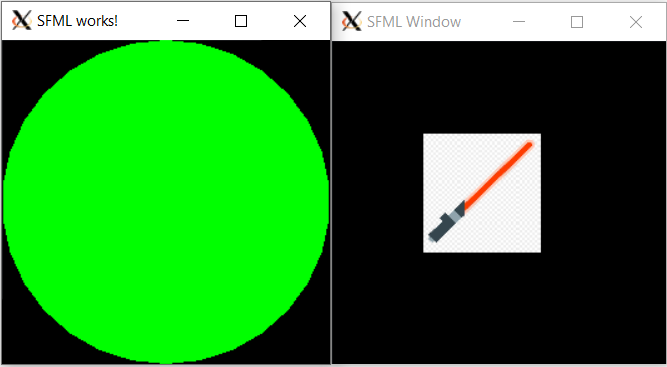
\includegraphics[width=0.5\columnwidth]{ps0_output}
\caption{PS0 Output}
\label{fig:output}
\end{figure}

\subsection{What I Already Knew}\label{sec:ps0:knew} % What was known prior to the assignment

Since this was an intro project, I only had my past C++ coding experience.

\subsection{Design Decisions and Implementations}\label{sec:ps0:decisions} % Important decisions or implementations I made

There were not many major decisions for this project as ti was a demo to learn SFML.
However, since I chose a lightsaber, I thought it was best that a noise to go along with the movement so I chose to do such.

\subsection{What I Learned}\label{sec:ps0:learned} % What I learned because of the assignment

I learned how to run a basic SFML program.
This included generating a window and drawing a sprite to that window.
I learned how to move a sprite using keystrokes which in turn could cause an action, in this cause making a noise.

\subsection{Challenges}\label{sec:ps0:challenges} % Challenges along the way and any that went unresolved

There were were no major complications along the way.

\newpage
\subsection{Codebase}\label{sec:ps0:code} % Code: Makefile, .cpp main, .hpp main, .cpp support, .hpp support, .cpp tests

\bigskip
\title{\large Makefile:}
\lstinputlisting{../ps0/Makefile}
\bigskip
\title{\large main.cpp:}
\lstinputlisting{../ps0/main.cpp} 
\section{PS1: Photomagic with LFSR}\label{sec:ps1}

\subsection{Overview}\label{sec:ps1:overview} % A discussion of the assignment itself

In this project, we were tasked with making a program that could encrypt and decrypt an image given a binary seed.
To do this, a class FibLFSR was made with similarities to a linear feedback shift register.
Using this class, an image's pixels could be randomized and the image could be 'encrypted'.  
Based off the design of the FibLFSR, an image could be encrypted and decrypted given the same seed was used.

\subsection{End Product}\label{sec:ps1:accomplish} % What I accomplished and images/results

Below is the output.
On the left is the encryption, from the Darth Vader image into seeming random 'static'.
On the right is the decryption, from 'static' back into the original Darth Vader image.

\begin{figure}[h]
\centering
\begin{minipage}[b]{0.4\textwidth}
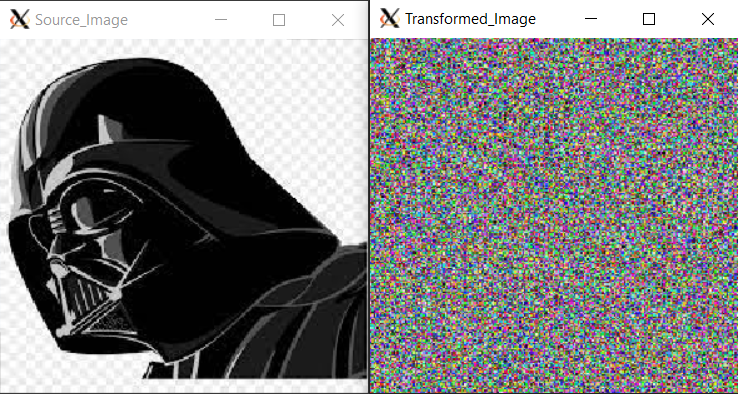
\includegraphics[width=\textwidth]{ps1-1_output}
\caption{Encryption}
\end{minipage}
\hfill
\begin{minipage}[b]{0.4\textwidth}
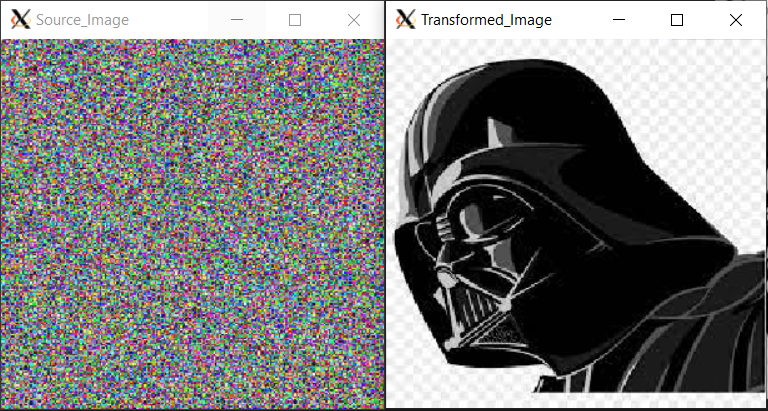
\includegraphics[width=\textwidth]{ps1-2_output}
\caption{Decryption}
\end{minipage}
\end{figure}

\subsection{What I Already Knew}\label{sec:ps1:knew} % What was known prior to the assignment

I knew how to shift bits and how shift registers worked for reference when creating the LibLFSR class.
I also knew how to make a window and draw to it in SFML from ps0.

\subsection{Design Decisions and Implementations}\label{sec:ps1:decisions} % Important decisions or implementations I made

I chose to represent the FibLFSR class as a string. 
This made it so accessing certain elements and appending or taking a character from the front to represent a shift wasn't too difficult.
Inside the class, the 'step' function was made to represent a shift.
This function XORed specific bit positions, with the final bit result being appended to the string, and the front bit being removed.
This was then used by 'generate' function to make a binary number of a given size.
The function looped for a given size and generated a bit until it had a string of bits and had created a number.
To encrypt/decrypt the image, the 'transform' function used this idea to randomize a given image's pixels.
Each pixel's rgb value could be represented as an 8-bit number so 'generate' was used with an argument of 8 to seemingly generate a completely random red, green, or blue value.
This made each pixel completely different from it's original rgb values.
\bigskip

As extra credit I made it so not only a binary seed could be used to encrypt the image, but a seed of any numbers or characters could be used.
For this, I accounted for any character located in the ASCII table.
What I did was make any odd characters in the ASCII table a 1 and any even a 0.
This made it so 0 and 1 still remained the same while other characters could now be made into 0s and 1s.
Any password over length 16 had those trailing bits ignored and anything shorter had it's remaining bits alternating between '0's and '1's.
These together make it seem as random as possible while also making it so the same alphanumeric seed made the same binary seed every time.

\subsection{What I Learned}\label{sec:ps1:learned} % What I learned because of the assignment

I learned how to run two windows simultaneously in SFML.
For an image, I learned how access and edit the rgb values of it's pixels.

\subsection{Challenges}\label{sec:ps1:challenges} % Challenges along the way and any that went unresolved

There were were no major complications along the way.

\newpage
\subsection{Codebase}\label{sec:ps1:code} % Code: Makefile, .cpp main, .hpp main, .cpp support, .hpp support, .cpp tests

\bigskip
\title{\large Makefile:}
\lstinputlisting{../ps1b/Makefile}
\bigskip
\title{\large Photomagic.cpp:}
\lstinputlisting{../ps1b/Photomagic.cpp}
\bigskip
\title{\large FibLFSR.cpp:}
\lstinputlisting{../ps1b/FibLFSR.cpp}
\bigskip
\title{\large FibLFSR.hpp:}
\lstinputlisting{../ps1b/FibLFSR.hpp}
\bigskip
\title{\large test.cpp:}
\lstinputlisting{../ps1b/test.cpp}

\newpage



\section{PS2: Sokoban}\label{sec:ps2}

\subsection{Overview}\label{sec:ps2:overview} % A discussion of the assignment itself

In this assignment, we were tasked with making a simple version of the game Sokoban which is a simple 2d block-pushing game.
The program was to be run with a given level file that contained a grid of characters representing the starting game state.
The game includes the ability of being able to move the player around using WASD and reset the level using 'R'. 
The boxes/storage containers are able to be pushed around the game area with the goal of putting them into the storage spaces.
Once all the boxes are in the storage spaces or all storage spaces are filled with boxes thed the game is won.

\subsection{End Product}\label{sec:ps2:accomplish} % What I accomplished and images/results

Below is the output.
Level one is being played.
On the left is the starting game state.
On the right is the game being won.

\begin{figure}[h]
\centering
\begin{minipage}[b]{0.4\textwidth}
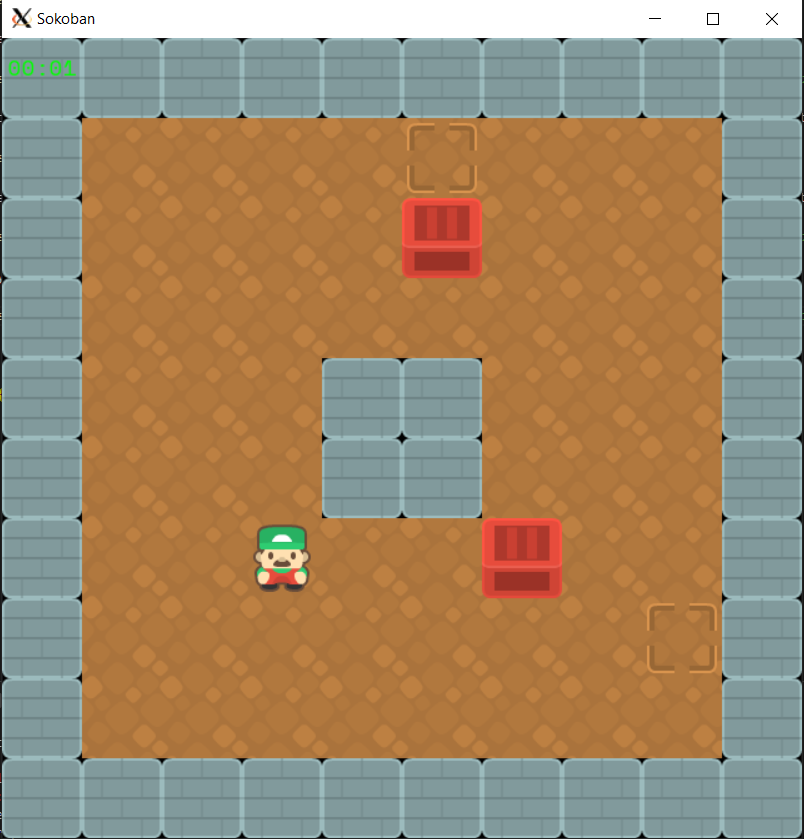
\includegraphics[width=\textwidth]{ps2-1_output}
\caption{Level 1 Start}
\end{minipage}
\hfill
\begin{minipage}[b]{0.4\textwidth}
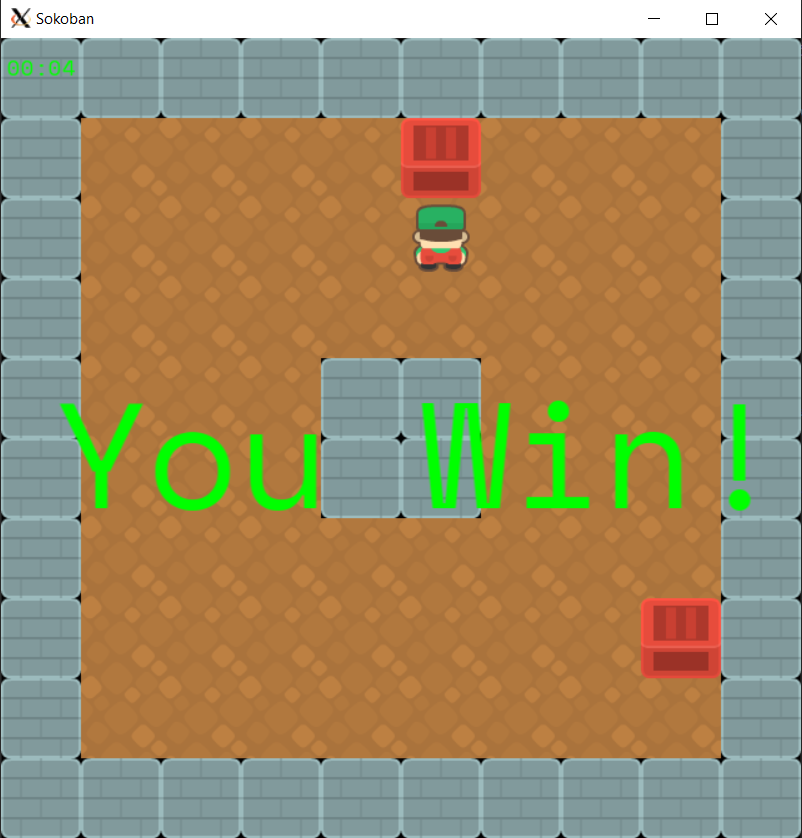
\includegraphics[width=\textwidth]{ps2-2_output}
\caption{Level 1 Won}
\end{minipage}
\end{figure}

\subsection{What I Already Knew}\label{sec:ps2:knew} % What was known prior to the assignment

I knew some basics of SFML for sprite movement and drawing to the screen.
As for C++, I knew a variety of containers that could be used to develop the class.
I also had past experience of implementing game mechanics/boundary conditions from previous school and personal projects.

\subsection{Design Decisions and Implementations}\label{sec:ps2:decisions} % Important decisions or implementations I made

For the game internals  I created a Sokoban class. To display the game, I separated the game field into many different object containers.
I first made a vector of textures that were loaded in once. 
These were to be shared between multiple sprites because sprites take up far less memory than textures, so this improved load speeds and reduced memory usage.
I then made a 2d vector of characters to hold an exact copy of level file. This was for ease of access later on for game mechanics. 
As for displaying the game, I separated the environment(walls and floors), storage containers/boxes, storage spots, and the player into different sprite containers.
This made it so that certain game elements could be drawn over each other/have same positions, such as the player standing on the floor. 
To display these, the class inherited from SFML draw class and the 'draw' function was overloaded so if you called 'draw' with a Sokoban object it would draw the whole game out.

\bigskip
As for the core game mechanics, I controlled most of them through the 'movePlayer' and 'isWon' functions.
In the 'movePlayer' function I made a vector of x,y pairs that represented the displacement after a key press.
This made it so I could generalize the game mechanics across keystroke presses to reduce the code four fold.
For each movement I checked that it wouldn't be an illegal movement and would act appropriately with the box.
For the player, that meant they could not go out of bounds, through a wall, or into a box.
However, the player should be allowed to push a box, unless another box was in front of it, or by pushing the box it would go out of bounds or through a wall.
If any such illegal movement was attempted, the 'movePlayer' made sure no such movement was made.
If there were no illegal actions being made the respective sprite's positions were updated.

\bigskip
In the isWon function there was a few scenarios where the player would win.
If there were equal boxes to spaces, or more boxes than spaces, the player won once all the storage spaces were filled. 
If there were more spaces than boxes, the player won once all the boxes were in a storage location.
To account for all of them the lower number between the number of boxes and the number of storage spaces could be used to determine when the game was won.
To check if boxes were in storage spaces I looped through the vectors of both. For each box/storage combination I compared their position using the 'find\_if' algorithm paired with a lambda function. 
If by the end of looping the number of boxes in storage spots met that determined lower number, then the player had won. 

\bigskip
For extra credit, I added a few different things.
I first added a timer in the top left that counted the time passed after the level began.
Some small features I added were a victory sound when the game was won, and a player model change when the player's direction changed.
As a custom feature I added the ability for the player to play the next level if 'N' is pressed or play the previous level if 'P' is pressed after completing current level.
To go to the next/previous level that level must exist or the game will just remain on the winning screen.

\subsection{What I Learned}\label{sec:ps2:learned} % What I learned because of the assignment

I continued learn more about SFML, especially sprites and their possible functions.
I learned how to properly overload the draw function for user made classes/objects.
I learned/used lambda functions for the first time.

\subsection{Challenges}\label{sec:ps2:challenges} % Challenges along the way and any that went unresolved

Everything turned out how I wanted it, but this was the first project with some more challenging problems.
The first big trouble I had was overloading the draw function;
it was simple after I completed it, but it was hard to find how to overload it properly using SFML API, so it became somewhat of a trial and error.
In general it was tough to figure out how I wanted my game to be represented, so I was constantly making more containers to hold the game objects.
In the gameplay part of the project, just eliminating all of the possible boundary conditions for movement took a little while.
The hardest challenge was trying to center the victory text, but  that too felt like was because of SFML API.

\newpage
\subsection{Codebase}\label{sec:ps2:code} % Code: Makefile, .cpp main, .hpp main, .cpp support, .hpp support, .cpp tests

\bigskip
\title{\large Makefile:}
\lstinputlisting{../ps2b/Makefile}
\bigskip
\title{\large main.cpp:}
\lstinputlisting{../ps2b/main.cpp}
\bigskip
\title{\large Sokoban.cpp:}
\lstinputlisting{../ps2b/Sokoban.cpp}
\bigskip
\title{\large Sokoban.hpp:}
\lstinputlisting{../ps2b/Sokoban.hpp}

\newpage

\section{PS3: Pythagorean Tree}\label{sec:ps3}

\subsection{Overview}\label{sec:ps3:overview} % A discussion of the assignment itself

This project creates a Pythagorean Tree from a given side length, size, and angle measure.
A Pythagorean Tree starts as a square, and generates two more squares (of possible different sizes depending on the given angle measure) in opposing directions.
Each new square will generate two new squares in the same manner as many times as the given recursion depth.

\subsection{End Product}\label{sec:ps3:accomplish} % What I accomplished and images/results

Below is the output.
This is the simplest version of the tree using a 45 degree angle.

\begin{figure}[h]
\centering
\begin{minipage}[b]{0.4\textwidth}
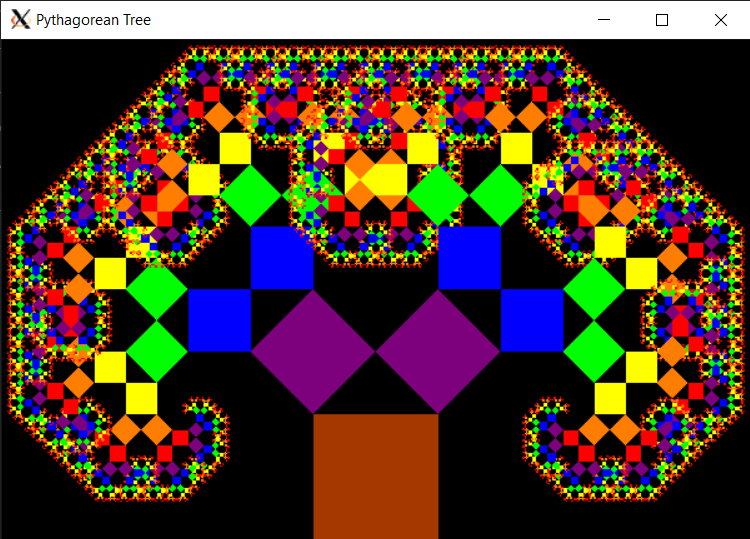
\includegraphics[width=\textwidth]{ps3-1_output}
\caption{Pythagorean Tree: 45 Degrees}
\end{minipage}
\end{figure}

\subsection{What I Already Knew}\label{sec:ps3:knew} % What was known prior to the assignment

I had SFML experience from past projects and basic manipulation fo rectangular shapes.
As for C++, I knew a how to create a basic tree and node class and use recursion within them.

\subsection{Design Decisions and Implementations}\label{sec:ps3:decisions} % Important decisions or implementations I made

I chose to make two classes, a Tree class and a Node class.
A tree object has a root Node which represents the starting square in this case.
Each Node is a rectangular sprite with the addition of a left and right node member to generate future squares.
The Tree calls upon a recursive 'grow' function which creates two children from a given parent Node with the correct new position, angle, size, etc.
This recursion loops for the given depth.

\bigskip
For extra credit, I added two things.
The first feature I added was color changing depening on the depth of the tree.
The starting color is always brown (like a stump) and then any following levels loop through the rainbow.
The second feature I added was the ability to chnage the angle of the new generated squares.
However, in doing so, a problem arose which is coverd in the challenges section.

\subsection{What I Learned}\label{sec:ps3:learned} % What I learned because of the assignment

I learned what a Pythagorean tree is and how it's made.
I learned more about SFML shapes and how translations effect them.

\subsection{Challenges}\label{sec:ps3:challenges} % Challenges along the way and any that went unresolved

I came across a few different challenges.
The first was setting the origin of every new object.
SFML API is pretty bad at documenting this, along with it being confusing in general, so it took me a while to get each new rotation/position correct.
The second, I was unable to fix, and was the problem resulting from doing the extra credit mentioned above which involves changing the angle of recursion.
With a changed angle the tree may no longer fully fit to the generated window.
I could not figure out a proper way to make a window that would prefectly fit any given generated tree to screen.

\newpage
\subsection{Codebase}\label{sec:ps3:code} % Code: Makefile, .cpp main, .hpp main, .cpp support, .hpp support, .cpp tests

\bigskip
\title{\large Makefile:}
\lstinputlisting{../ps3/Makefile}
\bigskip
\title{\large main.cpp:}
\lstinputlisting{../ps3/main.cpp}
\bigskip
\title{\large Sokoban.cpp:}
\lstinputlisting{../ps3/PTree.cpp}
\bigskip
\title{\large Sokoban.hpp:}
\lstinputlisting{../ps3/PTree.hpp}

\newpage

\section{ps4: Checkers}\label{sec:ps4}

\subsection{Overview}\label{sec:ps4:overview} % A discussion of the assignment itself

This project builds the widely known game of Checkers.
In this game, two players, black and red, look to remove each other's pieces by jumping over them.
When a player no longer ahs any piece on the game board the other player wins. 
During a player's turn they can select a piece and it will highlight the tiles where the piece can move.
A piece can move in two diagonal directions depending on the piece's color.
If that move includes jumping a piece, the piece that is jumped is removed from the game board.
If a piece arrives at the opposing players side that piece is 'kinged', and can now move in all four diagonal directions. 
The game mechanics that were not yet implemented were multi-jumping, and forcing a player to make a jump if they can.

\subsection{End Product}\label{sec:ps4:accomplish} % What I accomplished and images/results

Below is the output.
This is the standard setup for a Checkers game.

\begin{figure}[h]
\centering
\begin{minipage}[b]{0.4\textwidth}
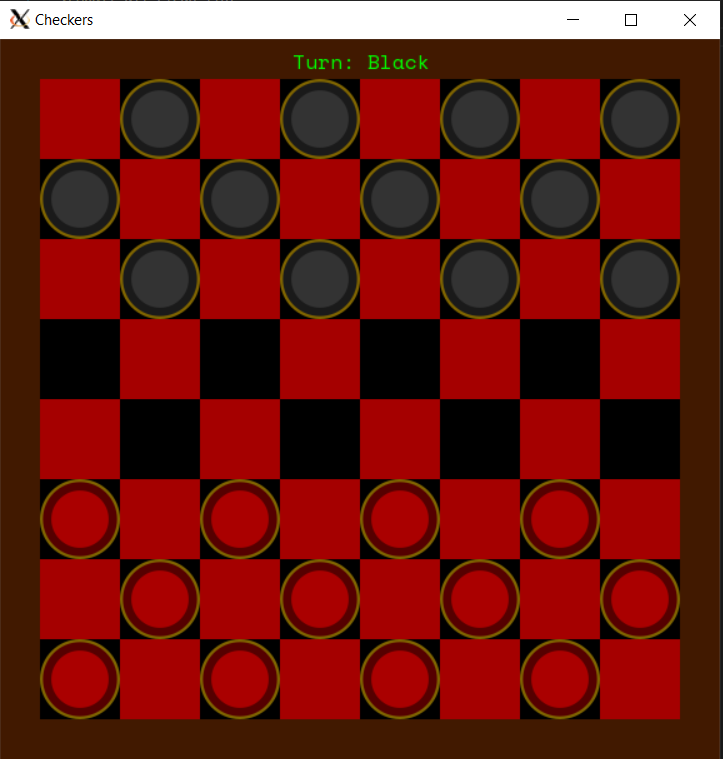
\includegraphics[width=\textwidth]{ps4-1_output}
\caption{Checkers: Start}
\end{minipage}
\end{figure}

\subsection{What I Already Knew}\label{sec:ps4:knew} % What was known prior to the assignment

Going into this project I had already completed Sokoban, so I had a good foundation for creating a game UI in SFML and implementing its game mechanics using C++.

\subsection{Design Decisions and Implementations}\label{sec:ps4:decisions} % Important decisions or implementations I made

The code for Checkers was comprised of two major classes called 'Checkers' and 'Pawn'.
The 'Pawn' class was meant to represent a piece and contained the sprite for a game piece along with a boolean that indicated if it was a king or not.
In the 'Checkers' class I made a a vector containing the game textures with similar reasoning to the textures vector in Sokoban.
The game tiles were represented using a 2d-vector of rectangles.
Each player's peieces were separated into their own respective vectors of 'Pawns', one representing the red player and the other the black.
The Checkers class also had a boolean variable named '\_blackTurn' to represent whose turn it was.

The game starts by creating a 'Checkers' object which does the following:
\begin{itemize}
\item Creates a base layer of brown which represents the board's border.
\item Fills the 2d-vector of tiles with alternated red and black squares.
\item Adds a black piece to its respective vector for every black square that was in the first three rows and adds a red piece to its respective vector for every red piece that was in the final three rows.
\end{itemize}

Once the game was made a number of smaller helper functions were made to reduce repeat code and code length.
Here are some of the more important ones:
\begin{itemize}
\item 'isBlackTurn' - Returns whose turn it is, black or red.
\item 'toTile' - Converts a pixel's coordinates to a tile location.
\item 'inBounds' - Checks if a piece's move is in bound.
\item 'getCurrPieces' \& 'getOppPieces' - Returns the current players pieces and the opposing players pieces depending on whose turn it is.
\item 'clearHighlights' - Clears any previously highlighted pieces/tiles.
\end{itemize}

As for the larger functions, these include many of the core game mechanics as follows: 
\begin{itemize}
\item 'takeTurn' - Switches the players turn.
\item 'checkKing' - Checks if a pawn needs to be kinged by checking if any piece has reached the opponents side, and if so, makes that piece a king.
\item 'onTile' - Checks if a piece can be found on a given tile by looping through a players' pieces and comparing their locations to the given tile.
\item 'clickPieces' - Highlights a tile if the current player clicked on their piece at that tile.
It gets the current players pieces and loops through, checking to see if the click was on a tile with their piece.
If one is found any past piece selection highlights are cleared and the new tile is highlighted.
\item 'showMoves' - Highlights the tiles where the current selected piece can possibly move.
It first checks what type of piece it is, and if it is a king, to know what direction it can move in.
It then loops through those directions to highlight the tiles it can actually move to.
It checks the two moves of jumping into a adjacent open space and jumping an opposing piece where no other piece is on the next tile.
Finally, the 'makeMove' function is called.
\item 'makeMove' - Moves a player's selected piece into a highlighted move area.
It first checks the game board for a selected/highlighted piece.
It then makes sure the player's mouse click is on the highlighted move location by to the mouse location.
If the mouse click matches a spot where the piece can move, the piece is set to that spot, the current turn is switched to the next player, and any highlights are cleared.
Finally, the 'removePieceJumped' function is called.
\item 'removePieceJumped' - Removes a piece from the game board if it was jumped using remove\_if.
It finds the displacement between the starting spot of a piece and the move it just made using .
It then uses a lambda to check if an opposing piece can be found at that displacement.
If found, remove\_if returns a new end iterator that the 'erase' member function of vector takes to remove the associated piece from the game board.
\end{itemize}

\subsection{What I Learned}\label{sec:ps4:learned} % What I learned because of the assignment

I learned a few small things, but what I was able to put into practice/learn was refactoring.
The internals of the game were originally comprised of many larger functions.
Once I got the code working, refactoring took place to clean everything up and reduce code.
This consisted of  condensing lines and creating helper functions. 
Once in place, the code flowed much nicer, was easier to follow, and was more efficient.

\subsection{Challenges}\label{sec:ps4:challenges} % Challenges along the way and any that went unresolved

Overall this wasn't that different from Sokoban, so there weren't many new big challenges, but there were some smaller challenges.
One problem that arose was the implementation of the 'remove\_if' algorithm.
A piece that had jumped another would occasionally duplicate itself because I wasn't properly implementing the 'remove\_if' algorithm.
Once I re-read the documentation on 'remove\_if' I was able to properly use it and reduce the duplication problem.

\newpage
\subsection{Codebase}\label{sec:ps4:code} % Code: Makefile, .cpp main, .hpp main, .cpp support, .hpp support, .cpp tests

\bigskip1
\title{\large Makefile:}
\lstinputlisting{../ps4b/Makefile}
\bigskip
\title{\large main.cpp:}
\lstinputlisting{../ps4b/main.cpp}
\bigskip
\title{\large Checkers.cpp:}
\lstinputlisting{../ps4b/Checkers.cpp}
\bigskip
\title{\large Checkers.hpp:}
\lstinputlisting{../ps4b/Checkers.hpp}

\newpage

\section{ps5: DNA Alignment}\label{sec:ps5}

\subsection{Overview}\label{sec:ps5:overview} % A discussion of the assignment itself

This project computes the optimal sequence alignment for two DNA strings.
It aligns two DNA sequences using a least cost method.

\subsection{End Product}\label{sec:ps5:accomplish} % What I accomplished and images/results

Below is the output.
This aligns two DNA strings with the cost of the total alignment at the top with the cost of each alignment as the last column.

\begin{figure}[h]
\centering
\begin{minipage}[b]{0.4\textwidth}
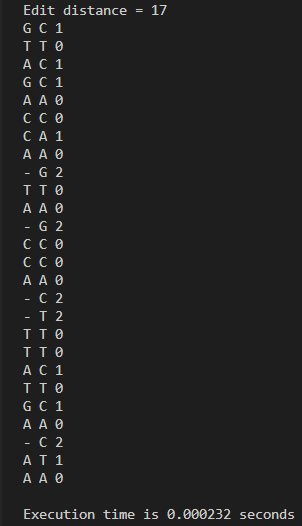
\includegraphics[width=\textwidth]{ps5-1_output}
\caption{"stx26" DNA Alignment}
\end{minipage}
\end{figure}

\subsection{What I Already Knew}\label{sec:ps5:knew} % What was known prior to the assignment

I knew how to create a matrix to store the cumulative penalties.

\subsection{Design Decisions and Implementations}\label{sec:ps5:decisions} % Important decisions or implementations I made

The project uses the Needleman-Wunsch of dynamic programming. 
It was implemented through the EDistance class, which takes two strings of length N and M, and creates an N x M matrix of integers.
To compute the value of each value in the matrix it was broken into sub-problems.
The final row and final column can be computed from the lengths of the given strings.
For filling everything else, we work backwards from the \[N\]\[M\] by filling it with the minimum of three values. 
These three values are the three possible cases: A letter of a string aligning with the same letter, a different letter, or a gap and finds the best comparison.
Once the matrix is filled, the penalty of alignment can be found at \[0\]\[0\].
The actual alignment can be traced backwards using a similar way we populated the matrix.

\subsection{What I Learned}\label{sec:ps5:learned} % What I learned because of the assignment

I learned what the Needleman-Wunsch dynamic programming method is and how it can be beneficial to reduce time complexity.

\subsection{Challenges}\label{sec:ps5:challenges} % Challenges along the way and any that went unresolved

There were no major challenge as the project guide layed ot a good foundation for writing the code.

\newpage
\subsection{Codebase}\label{sec:ps5:code} % Code: Makefile, .cpp main, .hpp main, .cpp support, .hpp support, .cpp tests

\bigskip
\title{\large Makefile:}
\lstinputlisting{../ps5/Makefile}
\bigskip
\title{\large main.cpp:}
\lstinputlisting{../ps5/main.cpp}
\bigskip
\title{\large Checkers.cpp:}
\lstinputlisting{../ps5/EDistance.cpp}
\bigskip
\title{\large Checkers.hpp:}
\lstinputlisting{../ps5/EDistance.hpp}

\newpage

\section{ps6: RandWriter}\label{sec:ps6}

\subsection{Overview}\label{sec:ps6:overview} % A discussion of the assignment itself

This project uses a given text and generates new random text based off of it.
It takes the text, a kgram length, and a new text length.
A kgram is a substring of the text of the given length.
Using these many many kgrams, and their occurrences, new text of any length can be generating using the past kgrams probabilities.

\subsection{End Product}\label{sec:ps6:accomplish} % What I accomplished and images/results

Below is the output.
This is a string of random text generated from the text provided by Tom Sawyer.
The kgram length was set to 7.
\bigskip
"CHAPTER VI MONDAY morning campfire.
He was literally hated and the old lady to call on Mrs.
Harper hugged and let's swear again in his brass door-knob"

\subsection{What I Already Knew}\label{sec:ps6:knew} % What was known prior to the assignment

I knew how to parse through text in C++..

\subsection{Design Decisions and Implementations}\label{sec:ps6:decisions} % Important decisions or implementations I made

This project created a RandWriter class which was used to hold the kgrams and k+1grams generated from a text. 
I chose to store the kgrams and k+1grams separately as unordered maps, where the key was a string representing the kgram, and the value was an int representing the number of times the kgram occurred.
The constructor parsed through the text and filled the two maps, while also generating a seed that would be used later for RNG.
As for the new text it goes as follows:
\begin{itemize}
\item 'generate' - This function returns a string of new text given a starting kgram and length of generation.
It loops for the desired length of generation, calls 'kRand' to get a pseudo-random character, and returns a string once all those characters have been generated.
\item 'kRand' - This function returns a character based of a given kgram.
The kgram is first checked to actually exist in the kgram map using the 'freq' function, and if it is, it finds and stores all its associated k+1grams.
It then counts the number of total occurrences of all k+1grams with kgram in them is that a k+1gram with more occurrences has a higher probability of being picked.
A number is then randomly generated based off the RandWrite seed, and a distribution is applied to it, so the random number is between 1 and the total occurrences. 
That random number is then used to pick one of the k+1grams.
That character is then taken and returned as the new random character.
\item 'freq' - Determines if a given kgram or a k+1gram can be found in their respective maps.
The overload for a k+1gram wasn't implemented because of how the internal structure of my RandWriter was made (two separate maps).
\end{itemize}

\subsection{What I Learned}\label{sec:ps6:learned} % What I learned because of the assignment

I learned what kgrams are.
I learned C++'s version of random number generation and how to implement that.
I learned more about maps and how to implement them.

\subsection{Challenges}\label{sec:ps6:challenges} % Challenges along the way and any that went unresolved

There were small challenges along the way, but nothing that became a major issue.

\newpage
\subsection{Codebase}\label{sec:ps6:code} % Code: Makefile, .cpp main, .hpp main, .cpp support, .hpp support, .cpp tests

\bigskip
\title{\large Makefile:}
\lstinputlisting{../ps6/Makefile}
\bigskip
\title{\large main.cpp:}
\lstinputlisting{../ps6/main.cpp}
\bigskip
\title{\large Checkers.cpp:}
\lstinputlisting{../ps6/RandWriter.cpp}
\bigskip
\title{\large Checkers.hpp:}
\lstinputlisting{../ps6/RandWriter.hpp}

\newpage

\section{ps7: Kronos Log Parsing}\label{sec:ps7}

\subsection{Overview}\label{sec:ps7:overview} % A discussion of the assignment itself

This project parses a log file using regular expressions and outputs a report file.

\subsection{End Product}\label{sec:ps7:accomplish} % What I accomplished and images/results

Below is the output.
This is the end portion of a report file.
It shows the final started and completed boots of a log file.
\bigskip
=== Device boot ===
41684(device5\_intouch.log): 2014-02-03 12:45:46 Boot Start
**** Incomplete boot **** 
\bigskip
=== Device boot ===
41694(device5\_intouch.log): 2014-02-03 14:02:34 Boot Start
41802(device5\_intouch.log): 2014-02-03 14:05:18 Boot Completed
	Boot Time: 164000ms

\subsection{What I Already Knew}\label{sec:ps7:knew} % What was known prior to the assignment

I knew how to parse through an input file in C++.

\subsection{Design Decisions and Implementations}\label{sec:ps7:decisions} % Important decisions or implementations I made

There wasn't a need for a class or an outside file so everything was done in main.
First two regex expressions were made to properly detect start and complete boots.
Each line from the log file was checked against tahese expressions.
When a boot started it was written to the report file with a date and time.
If a boot had already started and another boot was encountered before a complete boot an incomplete boot was written to the report file following the previous boot. 
The new boot was then written to the file with a date and time.
If a completion was encountered following a boot it was written to the file with a date and time.
The boot time between the start and completion was computed via the 'convertTime' function and was also added to the report.
This function took two date/time strings, made them ptime objects, subtracted them, and converted the computed time to milliseconds.
Once the whole log file was parsed, a summary was added to the beginning of the report indicating the total lines read, the total of boots started, and the total of completed boots.

\subsection{What I Learned}\label{sec:ps7:learned} % What I learned because of the assignment

I learned what regular expression were and how useful they are for parsing and finding important parts from large amount of data

\subsection{Challenges}\label{sec:ps7:challenges} % Challenges along the way and any that went unresolved

I had a little trouble at the start of where to start because it felt a bit daunting, but once I started it was pretty simple.
I also had some general trouble with the regex and time/date libraries because the API is really bad and hard to follow,
so some functions used from them took a second to get right.

\newpage
\subsection{Codebase}\label{sec:ps7:code} % Code: Makefile, .cpp main, .hpp main, .cpp support, .hpp support, .cpp tests

\bigskip
\title{\large Makefile:}
\lstinputlisting{../ps7/Makefile}
\bigskip
\title{\large main.cpp:}
\lstinputlisting{../ps7/main.cpp}
\bigskip
\title{\large Checkers.cpp:}
\lstinputlisting{../ps7/main.hpp}

\newpage


\end{document}